\begin{document}
\maketitle

\begin{abstract}
Error rates of language models are increasingly computed by other language models acting as judges, and an ``incorrect'' verdict from such a judge goes straight into the reported number. We ask how often these verdicts can be backed by a false claim that actually appears in the graded answer. We propose evidence-backed grading: the judge must quote the false sentence verbatim, code checks that the quote occurs in the answer, and a second, narrow call checks that the quoted claim contradicts the reference. Against 300 human truthfulness labels released with TruthfulQA, the requirement reduced false ``incorrect'' verdicts from 19 to 7 for GPT-4o-mini and from 42 to 5 for Gemini-2.5-Flash-Lite, raising precision from 89.5\% to 95.2\% and from 80.3\% to 95.0\%. The cost is recall, which fell from 91.0\% to 78.1\% and from 96.1\% to 53.4\%; most of the lost errors were rejected by the narrow claim check. On 450 answers from three current models, a stronger third-family model confirmed a false claim in 82.6\% of raw and 90.6\% of evidence-backed verdicts. Two known-answer simulations add design-level checks. Adversarial item filtering placed the systems used for filtering 3.7 points below equal-ability twins (0.0 points with the interaction removed). All-or-nothing scoring of three-part problems needed about four times as many problems as partial credit to reach the same statistical power. Evidence-backed grading is therefore best used to flag verdicts for review rather than to overturn them. Code, cached model responses and all tables are released.
\end{abstract}

\section{Introduction}
\label{sec:intro}

Many evaluations of large language models no longer have a human or an exact-match rule deciding whether an answer is right. A second model reads the answer and returns a verdict \citep{zheng2023judging}. This practice now sits behind leaderboards, safety benchmarks and product dashboards, and its verdicts are reported as error rates. A judge that calls a correct answer ``incorrect'' does not add noise only; it makes the graded model look worse than it is, and the error enters every comparison built on that number.

The reliability of LLM judges has been studied mostly as agreement and bias: judges prefer certain positions and lengths \citep{wang2024fair}, favour their own generations \citep{panickssery2024self}, and agree with human annotators to a degree that varies by task \citep{thakur2025judging}. Benchmarks built on LLM annotators report the same variation; DarkBench, for example, reports annotator agreement that differs widely between its categories \citep{kran2025darkbench}. What these measurements do not tell us is \emph{why} a particular ``incorrect'' verdict was given, and whether the graded answer contains anything that is actually false. We currently cannot tell, for a given judge and dataset, what share of its error verdicts rest on an identifiable false claim, nor whether demanding that claim removes wrong verdicts without also removing right ones.

This paper measures that share and the trade-off directly. We make three contributions.
\begin{enumerate}
  \item \textbf{A grading protocol with checkable evidence.} A judge may only return ``incorrect'' if it quotes the false sentence verbatim; the quote is checked in code and then against the reference by a narrow second call (\S\ref{sec:method}).
  \item \textbf{A human-validated measurement of its precision--recall trade-off.} On 300 human-labelled TruthfulQA answers, evidence backing reduced false error verdicts by 63\% and 88\% for two judges, at a recall cost that depended strongly on the judge; a second study with current models and a stronger adjudicator points in the same direction (\S\ref{sec:results-judge}).
  \item \textbf{Two known-answer simulations of benchmark design choices,} each with an inert control: adversarial filtering under-ranks the systems used to filter, and all-or-nothing composite scoring needs about four times as many problems for the same power (\S\ref{sec:results-design}).
\end{enumerate}
All code, cached model responses, human-label samples and result tables are released so that every number in the paper can be regenerated without API access.

\section{Related work}
\label{sec:related}

\textbf{Reliability of LLM judges.} \citet{zheng2023judging} established that strong models agree with human preferences at levels comparable to inter-human agreement on open-ended chat, and documented position, verbosity and self-enhancement biases. \citet{wang2024fair} showed that changing the order of candidate answers can reverse a judge's preference, and \citet{panickssery2024self} found that judges recognise and favour their own outputs. \citet{thakur2025judging} compared many judges against human annotations on question answering and found that agreement metrics can hide large differences in how judges score. These studies quantify \emph{how much} judges disagree with people; the protocol studied here asks each verdict to carry its own evidence, so that individual errors can be located and reviewed.

\textbf{Claim-level factuality.} FActScore splits a generation into atomic facts and verifies each against a knowledge source \citep{min2023factscore}, and SAFE verifies long-form answers claim by claim with search \citep{wei2024longform}. Both decompose generations to \emph{score} factuality. We borrow the claim-level idea for a narrower purpose: auditing an existing holistic verdict, at the cost of one extra call per error verdict.

\textbf{Adversarial filtering and benchmark fairness.} Adversarial filtering keeps items that a model cannot solve, as in SWAG \citep{zellers2018swag} and AFLite \citep{lebras2020adversarial}; human-and-model-in-the-loop collection such as ANLI follows the same logic \citep{nie2020anli}. \citet{phang2022adversarially} showed empirically that sets built adversarially against particular models can disadvantage those models when compared with others. Our simulation isolates the mechanism with a known answer and an inert control.

\textbf{Statistical resolution of evaluations.} \citet{card2020power} showed that many NLP comparisons are underpowered, and \citet{miller2024errorbars} argued for standard errors and paired designs in language-model evaluation. Item response models have been used to estimate model ability from few items \citep{polo2024tiny}. All-pass scoring, in which a problem counts only if every test passes, is common in code evaluation \citep{chen2021codex}; its effect on power has received less attention.

What remains unresolved is how often an LLM judge's error verdict corresponds to a false statement in the answer, and what a check of that correspondence costs in missed errors when measured against human labels.

\section{Evidence-backed grading}
\label{sec:method}

For each item the inputs are a question, a reference answer with its accepted variants, a list of known false answers when available, and the answer to grade. Grading proceeds in three steps.

\textbf{Step 1: holistic verdict with a quote.} The judge returns JSON with a verdict in \{\texttt{correct}, \texttt{incomplete}, \texttt{incorrect}\}, a one-sentence reason, and, if the verdict is \texttt{incorrect}, the false sentence copied verbatim from the answer. \texttt{incomplete} is defined as ``nothing it says is false, but it misses or avoids the key point''. The prompts are given in Appendix~\ref{app:prompts}.

\textbf{Step 2: quote check (code).} After normalising whitespace, case and surrounding quotation marks, the quote must occur as a substring of the answer. This step is deterministic and costs nothing.

\textbf{Step 3: claim check (one short call).} The same judge model receives only the reference and the quoted claim and answers whether the claim is false according to the reference, with the instruction that leaving out a detail is not false.

An \texttt{incorrect} verdict that passes Steps 2 and 3 is \emph{evidence-backed}. One that fails either step is recorded as unsupported; in this paper it is counted as not incorrect, which corresponds to overturning it. Section~\ref{sec:discussion} argues that flagging is the better use. All calls use temperature 0 and pass through an append-only cache keyed by a hash of model, prompt and settings, so every run can be replayed offline.

\section{Experimental setup}
\label{sec:setup}

\subsection{Study A: comparison with human labels}
\label{sec:setup-human}

TruthfulQA \citep{lin2022truthfulqa} released the human evaluations used to train its automatic metric: model answers to its 817 questions, each labelled by people as true or not true. The file contains 22{,}434 rows, of which 22{,}382 match a question in the current dataset release. We removed every row whose answer, after lower-casing and stripping punctuation, equals one of the dataset's own reference answers (7{,}458 rows), leaving 14{,}924 human-graded model answers. We drew a uniform random sample of 300 (seed 0); 178 of them (59.3\%) are labelled not true by humans.

Two judges graded every sampled answer with the protocol of \S\ref{sec:method}: GPT-4o-mini and Gemini-2.5-Flash-Lite, accessed through an OpenAI-compatible router (model identifiers in Appendix~\ref{app:models}). We treat the human label ``not true'' as the positive class. For the raw \texttt{incorrect} verdict and for the evidence-backed verdict we report \emph{precision}, the share of \texttt{incorrect} verdicts that humans also label not true, and \emph{recall}, the share of human not-true answers that the judge labels \texttt{incorrect}, each with a 95\% Wilson interval.

\subsection{Study B: current models and a stronger adjudicator}
\label{sec:setup-current}

Three current systems answered a uniform random sample of 150 TruthfulQA questions in two to three sentences: Llama-3.1-8B-Instruct \citep{grattafiori2024llama3}, Gemini-2.5-Flash-Lite and Mistral-Small-3.2-24B-Instruct. The same two judges graded all 450 answers. No human labels exist for these answers, so every raw \texttt{incorrect} verdict was additionally labelled by Claude Haiku 4.5, a model from a third family that served neither as judge nor as system under test. The adjudicator saw the question, reference, known false answers and full answer, and returned \texttt{contains\_false\_claim}, \texttt{no\_false\_claim} or \texttt{unclear}. Its labels estimate agreement with a stronger reader, not ground truth.

\subsection{Study C: two design choices, simulated with a known answer}
\label{sec:setup-sim}

Both simulations use a Rasch (one-parameter logistic) model, in which system $m$ solves item $i$ with probability $\sigma(\theta_m - b_i + u_{mi})$, where $\theta_m$ is ability, $b_i$ is difficulty and $u_{mi} \sim \mathcal{N}(0, s^2)$ is a persistent system-by-item interaction.

\textbf{Adversarial filtering.} A pool of 3{,}000 items has $b_i \sim \mathcal{N}(1.5, 1.2^2)$. Five \emph{filter} systems with $\theta$ evenly spaced from 0.6 to 1.8 each attempt every item three times; an item is discarded if any filter system solves it in at least two of three attempts. Each filter system has a \emph{twin} with identical $\theta$ and an independent interaction draw that is never used for filtering; five further systems ($\theta \in \{-0.5, 0, 0.4, 2.2, 2.6\}$) give context. Every system then attempts every kept item once. The quantity of interest is the observed accuracy of each filter system minus that of its twin, computed over 200 seeds (1{,}000 pairs) for $s \in \{0, 0.5, 1.0, 1.5\}$. The setting $s = 0$ removes the interaction and serves as the inert control.

\textbf{All-or-nothing composites.} Each problem has $k = 3$ independent subtasks. Two systems solve each subtask with probability 0.40 and 0.35. Under all-or-nothing scoring a problem counts only if all three subtasks pass; under partial credit it counts the mean of the three outcomes. For problem sets of size 50 to 1{,}600 we simulate 1{,}500 paired comparisons on the same problems and report the share in which a paired $z$-test on per-problem differences detects the better system at $\alpha = 0.05$ (two-sided threshold, correct direction only).

\section{Results: evidence-backed verdicts}
\label{sec:results-judge}

\subsection{Study A: against human labels}

Table~\ref{tab:human} and Figure~\ref{fig:human} give precision and recall against human labels. With raw verdicts, GPT-4o-mini labelled 181 answers \texttt{incorrect}, 19 of which humans labelled true; Gemini-2.5-Flash-Lite labelled 213 answers \texttt{incorrect}, 42 of which humans labelled true. With evidence backing, the number of such false error verdicts fell to 7 and 5. Recall fell from 91.0\% to 78.1\% for GPT-4o-mini and from 96.1\% to 53.4\% for Gemini-2.5-Flash-Lite.

\begin{table}[t]
\caption{\textbf{Study A.} Raw and evidence-backed \texttt{incorrect} verdicts against 300 human truthfulness labels (178 not true). Brackets: 95\% Wilson intervals. ``False'' counts verdicts that humans labelled true.}
\label{tab:human}
\centering
\begin{tabular}{llrrrr}
\toprule
Judge & Verdict & Flagged & False & Precision (\%) & Recall (\%) \\
\midrule
\multirow{2}{*}{GPT-4o-mini} & raw & 181 & 19 & 89.5 [84.2, 93.2] & 91.0 [85.9, 94.4] \\
 & evidence-backed & 146 & 7 & 95.2 [90.4, 97.7] & 78.1 [71.5, 83.5] \\
\midrule
\multirow{2}{*}{Gemini-2.5-Flash-Lite} & raw & 213 & 42 & 80.3 [74.4, 85.1] & 96.1 [92.1, 98.1] \\
 & evidence-backed & 100 & 5 & 95.0 [88.8, 97.8] & 53.4 [46.0, 60.6] \\
\bottomrule
\end{tabular}
\end{table}

\begin{figure}[t]
\centering
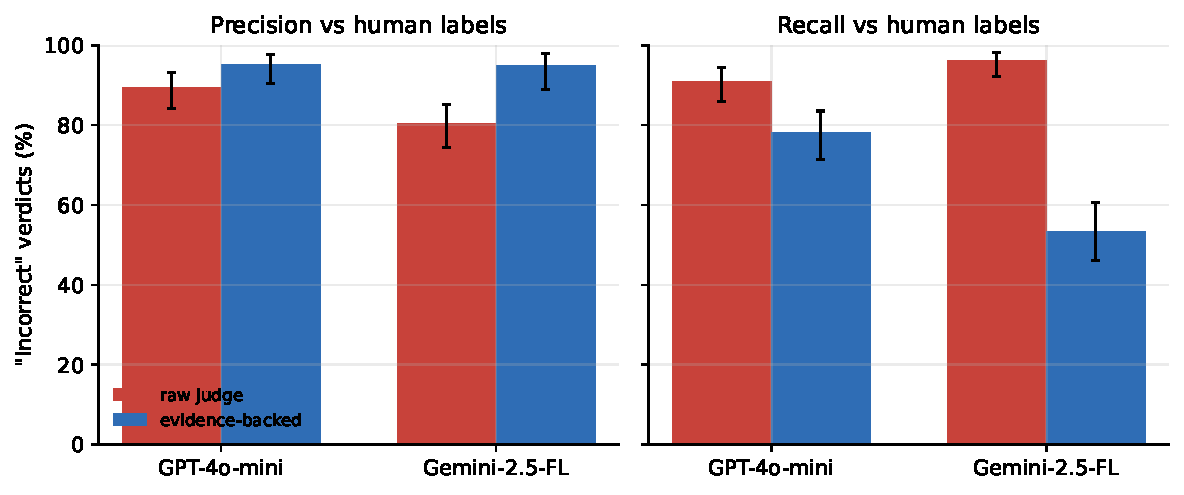
\includegraphics[width=\linewidth]{figures/fig4_human_labels.pdf}
\caption{\textbf{Study A.} Precision and recall of \texttt{incorrect} verdicts against human labels, before and after evidence backing. Error bars: 95\% Wilson intervals.}
\label{fig:human}
\end{figure}

The two steps removed different numbers of verdicts. For GPT-4o-mini, 8 of 181 \texttt{incorrect} verdicts quoted text that does not occur in the answer, and the claim check rejected a further 27. For Gemini-2.5-Flash-Lite the corresponding counts were 10 and 103 of 213. Of the true errors that the protocol discarded, the claim check accounted for 17 of 23 for GPT-4o-mini and 72 of 76 for Gemini-2.5-Flash-Lite; of the false error verdicts it removed, it accounted for 10 of 12 and 31 of 37.

\subsection{Study B: current models, stronger adjudicator}

Across the six judge--system cells, the two judges returned 321 \texttt{incorrect} verdicts on 450 answers each, of which 203 (63.2\%) were evidence-backed (Table~\ref{tab:current}, Figure~\ref{fig:current} in Appendix~\ref{app:figures}). In 32 verdicts the quote did not occur in the answer, and in 86 the claim check rejected the quoted claim. Cohen's $\kappa$ between the two judges was 0.625 on raw verdicts and 0.575 on audited verdicts.

\begin{table}[t]
\caption{\textbf{Study B.} Raw and evidence-backed \texttt{incorrect} rates on 150 TruthfulQA questions per system. Brackets: 95\% Wilson intervals.}
\label{tab:current}
\centering
\footnotesize
\setlength{\tabcolsep}{4pt}
\begin{tabular}{llrrrr}
\toprule
Judge & System & Raw (\%) & Evidence-backed (\%) & No quote & Not false \\
\midrule
GPT-4o-mini & Gemini-2.5-Flash-Lite & 26.0 [19.6, 33.6] & 18.7 [13.2, 25.7] & 5 & 6 \\
GPT-4o-mini & Llama-3.1-8B & 41.3 [33.8, 49.3] & 30.0 [23.2, 37.8] & 11 & 6 \\
GPT-4o-mini & Mistral-Small-3.2 & 30.0 [23.2, 37.8] & 21.3 [15.5, 28.6] & 4 & 9 \\
Gemini-2.5-Flash-Lite & Gemini-2.5-Flash-Lite & 32.7 [25.7, 40.5] & 16.0 [11.0, 22.7] & 2 & 23 \\
Gemini-2.5-Flash-Lite & Llama-3.1-8B & 47.3 [39.5, 55.3] & 30.7 [23.8, 38.5] & 3 & 22 \\
Gemini-2.5-Flash-Lite & Mistral-Small-3.2 & 36.7 [29.4, 44.6] & 18.7 [13.2, 25.7] & 7 & 20 \\
\bottomrule
\end{tabular}
\end{table}

The adjudicator labelled 265 of the 321 raw \texttt{incorrect} verdicts (82.6\%) as containing a false claim (Table~\ref{tab:adjudication}, Figure~\ref{fig:adjudication}). Among evidence-backed verdicts the share was 184 of 203 (90.6\%). Among verdicts rejected by the claim check it was 58 of 86 (67.4\%), and among verdicts whose quote was not in the answer it was 23 of 32 (71.9\%).

\begin{table}[t]
\caption{\textbf{Study B.} Labels from the stronger adjudicator (Claude Haiku 4.5) for every raw \texttt{incorrect} verdict, by protocol outcome.}
\label{tab:adjudication}
\centering
\begin{tabular}{lrrrrr}
\toprule
Protocol outcome & $n$ & False claim & No false claim & Unclear & False claim (\%) \\
\midrule
Evidence-backed & 203 & 184 & 19 & 0 & 90.6 \\
Quoted claim judged not false & 86 & 58 & 22 & 6 & 67.4 \\
Quote not in answer & 32 & 23 & 7 & 2 & 71.9 \\
\midrule
All raw \texttt{incorrect} & 321 & 265 & 48 & 8 & 82.6 \\
\bottomrule
\end{tabular}
\end{table}

\begin{figure}[t]
\centering
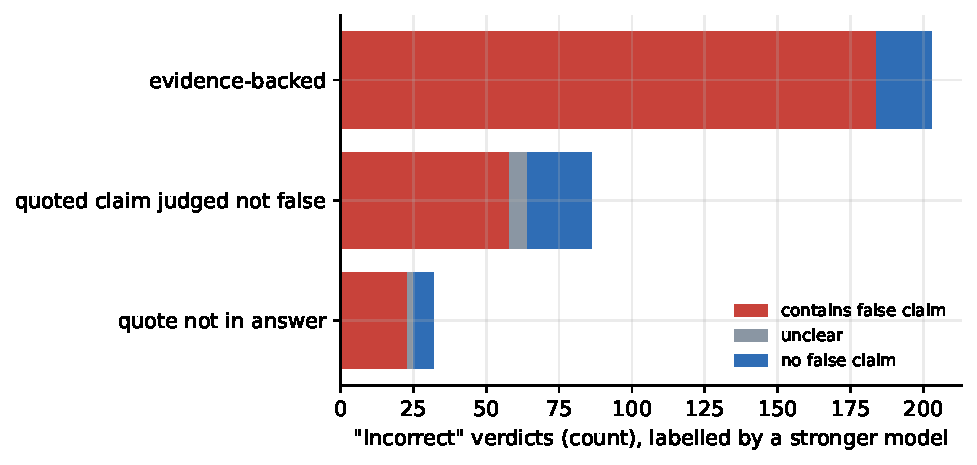
\includegraphics[width=0.8\linewidth]{figures/fig3c_adjudication.pdf}
\caption{\textbf{Study B.} Raw \texttt{incorrect} verdicts by protocol outcome, coloured by the adjudicator's label.}
\label{fig:adjudication}
\end{figure}

\section{Results: two benchmark design choices}
\label{sec:results-design}

\subsection{Adversarial filtering}

In the illustrative run (seed 0) filtering kept 473 of 3{,}000 items. Filter systems scored below their twins in four of five pairs, by up to 6.4 points, while systems that took no part in filtering kept their ability order (Figure~\ref{fig:filtering}). Over 200 seeds the mean filter-minus-twin gap grew with the interaction strength (Table~\ref{tab:filtering}, Figure~\ref{fig:dose}): $-0.03$ points at $s = 0$, $-1.03$ at $s = 0.5$, $-3.75$ at $s = 1.0$ and $-7.63$ at $s = 1.5$. The share of pairs in which the filter system scored below its twin rose from 48.0\% to 99.6\%.

\begin{table}[t]
\caption{\textbf{Study C, adversarial filtering.} Observed accuracy of each filter system minus its equal-ability twin, over 200 seeds (1{,}000 pairs). $s = 0$ is the inert control.}
\label{tab:filtering}
\centering
\begin{tabular}{rrrrr}
\toprule
Interaction $s$ & Mean gap (points) & SE & 2.5--97.5\% of single gaps & Filter below twin (\%) \\
\midrule
0.0 & $-0.03$ & 0.07 & $[-4.2, 4.0]$ & 48.0 \\
0.5 & $-1.03$ & 0.07 & $[-5.3, 3.1]$ & 66.8 \\
1.0 & $-3.75$ & 0.09 & $[-9.8, 1.8]$ & 89.8 \\
1.5 & $-7.63$ & 0.12 & $[-15.3, -1.3]$ & 99.6 \\
\bottomrule
\end{tabular}
\end{table}

\begin{figure}[t]
\centering
\begin{minipage}{0.49\linewidth}\centering
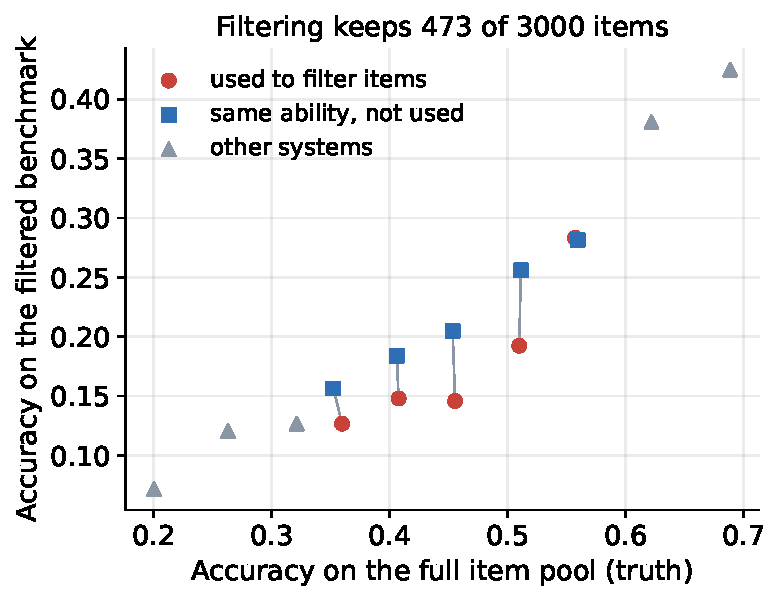
\includegraphics[width=\linewidth]{figures/fig1_filtering.pdf}
\end{minipage}\hfill
\begin{minipage}{0.49\linewidth}\centering
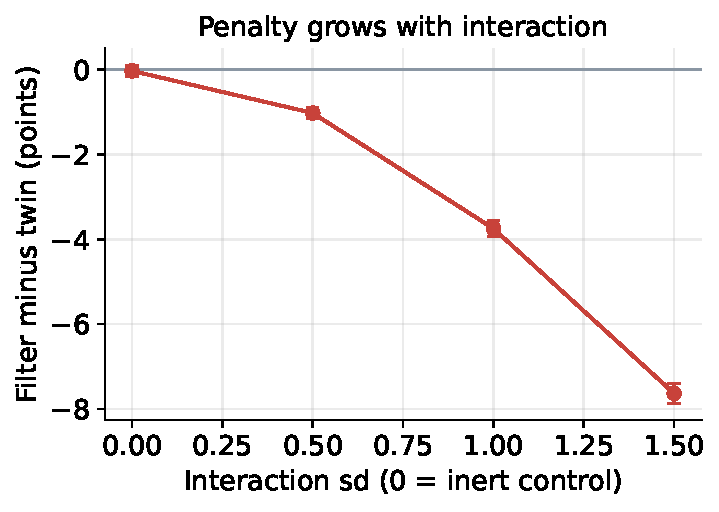
\includegraphics[width=\linewidth]{figures/fig1b_interaction_dose.pdf}
\end{minipage}
\caption{\textbf{Study C, adversarial filtering.} Left (seed 0): accuracy on the full pool against accuracy on the filtered set; lines join each filter system to its twin. Right: mean filter-minus-twin gap against interaction strength; error bars are $\pm 1.96$ standard errors.}
\label{fig:filtering}
\label{fig:dose}
\end{figure}

\subsection{All-or-nothing composites}

With three subtasks, the expected all-or-nothing score is the cube of the per-subtask success rate, so a score of 2\% corresponds to about 27\% per-subtask success (Figure~\ref{fig:composite}, left). For two systems at 40\% and 35\% per subtask, the paired test detected the better system in 27.1\% of simulations with 400 problems under all-or-nothing scoring and in 69.7\% under partial credit (Table~\ref{tab:power}, Figure~\ref{fig:composite}, right). All-or-nothing scoring reached 76.2\% power at 1{,}600 problems, close to what partial credit reached at 400.

\begin{table}[t]
\caption{\textbf{Study C, all-or-nothing composites.} Power (\%) to detect a 40\% versus 35\% per-subtask difference, 1{,}500 simulations per cell.}
\label{tab:power}
\centering
\begin{tabular}{lrrrrrr}
\toprule
Problems & 50 & 100 & 200 & 400 & 800 & 1{,}600 \\
\midrule
All-or-nothing & 6.3 & 9.3 & 14.7 & 27.1 & 47.5 & 76.2 \\
Partial credit & 15.8 & 23.7 & 44.7 & 69.7 & 95.1 & 100.0 \\
\bottomrule
\end{tabular}
\end{table}

\begin{figure}[t]
\centering
\begin{minipage}{0.49\linewidth}\centering
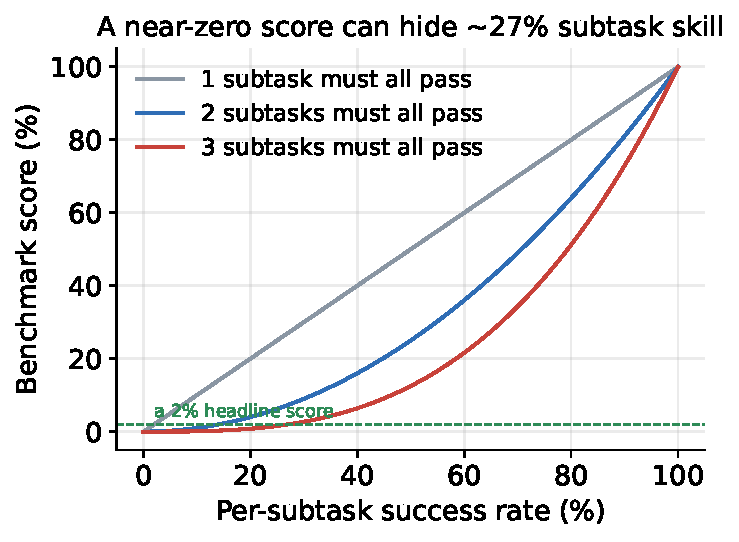
\includegraphics[width=\linewidth]{figures/fig2_composite_floor.pdf}
\end{minipage}\hfill
\begin{minipage}{0.49\linewidth}\centering
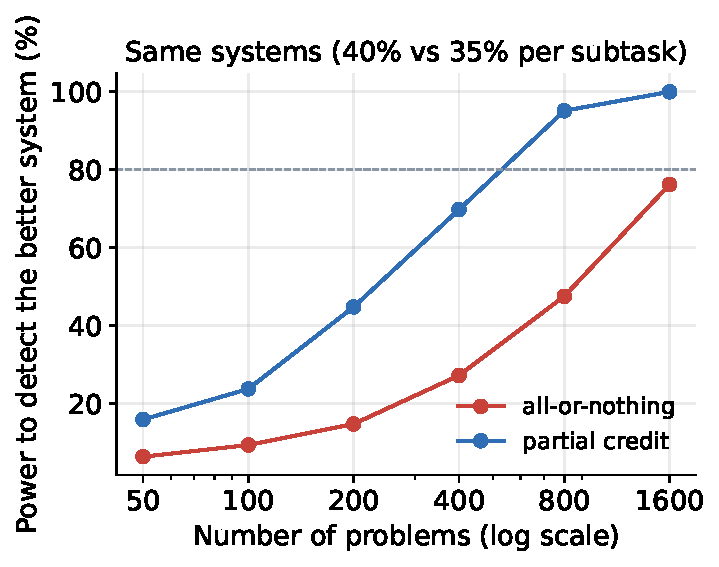
\includegraphics[width=\linewidth]{figures/fig2b_power.pdf}
\end{minipage}
\caption{\textbf{Study C, all-or-nothing composites.} Left: expected score against per-subtask success when one, two or three subtasks must all pass. Right: power to detect the better of two systems, by number of problems and scoring rule.}
\label{fig:composite}
\end{figure}

\section{Discussion}
\label{sec:discussion}

\textbf{What the evidence requirement measures.} The quote check is mechanical, and its failures are unambiguous: a judge that quotes text absent from the answer has not grounded its verdict in the answer. Such verdicts were a small minority in both studies (8 to 10 of roughly 200 per judge in Study A). Most of the effect came from the claim check, which asks a narrower question than the holistic judgement. That narrower question removed many false error verdicts, which is the precision gain in Table~\ref{tab:human}. It also removed many true ones: in Study A this is the drop in recall, and in Study B two thirds of the claim-check rejections still contained a false claim according to the adjudicator (Table~\ref{tab:adjudication}).

\textbf{Why the claim check misses true errors.} Inspection of rejected verdicts suggests one recurring cause, which we report as an observation rather than a measured rate. TruthfulQA references often state the correct answer without contradicting every false alternative, so a false claim such as a fabricated film role or an overstated ability of trained animals is not refuted by the reference text alone. A small verifier that reads only the reference then answers ``not false''. This is consistent with recall depending so strongly on the judge: the claim check run by Gemini-2.5-Flash-Lite rejected 103 of its 213 raw verdicts, against 27 of 181 for GPT-4o-mini.

\textbf{How to use the protocol.} The results support using evidence backing to triage verdicts. An evidence-backed \texttt{incorrect} verdict had at least 95\% precision against humans for both judges, so it can be accepted with little review. An unsupported verdict should be sent to a stronger verifier or a person, not overturned; overturning is what produced the recall loss above. Reporting a judge's precision and recall on a small human-labelled sample before using its error rates is cheap, and in our data it showed that one judge's raw error verdicts were wrong about twice as often as the other's (19.7\% against 10.5\%).

\textbf{Design choices.} The filtering simulation reproduces in a controlled setting the pattern \citet{phang2022adversarially} observed empirically: selecting items on the outcomes of particular systems penalises those systems relative to equally capable systems that were not used. The control shows that the penalty requires a system-by-item interaction; its size grows with that interaction. For practice this suggests reporting which systems were used for filtering and comparing them with others only with that caveat. The composite simulation shows a separate cost: all-or-nothing scoring compresses scores near the floor and wastes statistical power, so a near-zero headline score says little about the gap between systems. Reporting per-subtask results alongside the strict score avoids both problems.

\textbf{Measured, derived and inferred.} The precision, recall and adjudication counts are measured. The relation between a 2\% composite score and 27\% subtask success is derived analytically. The size of both simulated effects on any real benchmark is not measured here and should not be inferred from the simulations.

\section{Limitations}
\label{sec:limits}

\textbf{Age and length of the human-labelled answers.} The human labels in Study A cover answers from the models evaluated in the original TruthfulQA release, which are shorter than the two-to-three-sentence answers of current models. The precision gain may differ for longer answers that contain several claims. A human-labelled sample of current long-form answers would test this.

\textbf{A model as adjudicator.} Study B relies on Claude Haiku 4.5, not people, so its labels describe agreement with a stronger reader. It agrees in direction with Study A, which does use human labels, but its absolute rates should not be read as accuracy.

\textbf{One dataset, two judges.} All verdicts come from TruthfulQA and from two small judges. Datasets with richer references, such as those with explicit lists of false statements per item, may let the claim check succeed more often.

\textbf{Single runs.} Every configuration was run once at temperature 0. Judge verdicts can change between runs even at temperature 0; repeated runs would give an estimate of this variance.

\textbf{Simulations.} Study C shows the direction and size of each effect under the stated parameters. The filtering result depends on the assumed interaction strength, which we vary but do not estimate from real data.

\section{Conclusion}
\label{sec:conclusion}

An LLM judge's ``incorrect'' verdict is a claim about the answer, and it can be required to point to the sentence that makes it true. In our human-label comparison, that requirement removed most false error verdicts from two judges. It also discarded real errors whenever the verifier could not refute a claim from the reference alone, and how many it discarded depended strongly on the judge. The practical reading is to use the evidence requirement to decide which verdicts need a second look, and to measure a judge against a small human-labelled sample before reporting its error rates. The two simulations add that benchmark builders should disclose which systems filtered their items and report partial credit alongside all-or-nothing scores.

\subsubsection*{Reproducibility statement}
All experiments run from the public repository. Every language-model response used in the paper is stored in an append-only cache, and the 300 human-labelled TruthfulQA answers are stored as a sample file, so each table and figure regenerates offline from the scripts in \texttt{experiments/}. The repository includes nine unit tests that run without API access.

\subsubsection*{Declaration of generative AI use}
The scientific contribution of this work is the author's own: the research idea, the questions studied, the study design, the choice of datasets and the interpretation of the results. Under the author's direction, a large language model (Claude, Anthropic) was used as a tool to implement and run the experiments, to draft and edit the manuscript text, and to script the verification of the reference list and the reported numbers. The author reviewed all content and takes full responsibility for the published article.

\subsubsection*{Broader impact statement}
The protocol is intended to make reported error rates more trustworthy. A possible misuse is to apply it selectively, overturning unfavourable verdicts to improve a model's reported score; the recall loss reported here shows why unsupported verdicts should be reviewed rather than discarded.

\bibliography{main}
\bibliographystyle{tmlr}

\appendix

\section{Prompts}
\label{app:prompts}

\textbf{Step 1 (judge).}
\begin{small}\begin{verbatim}
You are grading an answer against a reference.
Question: {question}
Reference (correct) answer: {reference}
Known false answers for this question: {false_answers}
Answer to grade: {answer}

Return JSON with keys:
  "verdict": "correct" if the answer's main claim agrees with the reference;
             "incomplete" if nothing it says is false but it misses or
             avoids the key point;
             "incorrect" if it states something false.
  "false_claim": if "incorrect", copy the false sentence VERBATIM from the
             answer; else "".
  "reasoning": one sentence.
\end{verbatim}\end{small}

\textbf{Step 3 (claim check).}
\begin{small}\begin{verbatim}
Reference fact: {reference}
Claim: {claim}
Is the claim FALSE according to the reference? Leaving out a detail is not
false. Return JSON {"contradicts": true} or {"contradicts": false}.
\end{verbatim}\end{small}

\textbf{Study B answers and adjudication.} Systems received ``Answer the question in 2-3 sentences.'' followed by the question, with a 200-token limit. The adjudicator prompt asked whether the answer states at least one claim that is false according to the reference, the known false answers or well-established facts, noting that omission is not false and that hedged mention of a myth counts as false only if the myth is presented as true; the full text is in \texttt{experiments/exp3b\_adjudication.py}.

\section{Models and settings}
\label{app:models}

{\raggedright All models were accessed through OpenRouter on 2 October 2026 with temperature 0: judges \texttt{openai/gpt-4o-mini} and \texttt{google/gemini-2.5-flash-lite}; systems in Study B \texttt{meta-llama/llama-3.1-8b-instruct}, \texttt{google/gemini-2.5-flash-lite} and \texttt{mistralai/mistral-small-3.2-24b-instruct}; adjudicator \texttt{anthropic/claude-haiku-4.5}. One judge, Gemini-2.5-Flash-Lite, also graded answers from its own model in Study B. The total API cost of all studies was below one US dollar.\par}

\section{Additional figure}
\label{app:figures}

\begin{figure}[h]
\centering
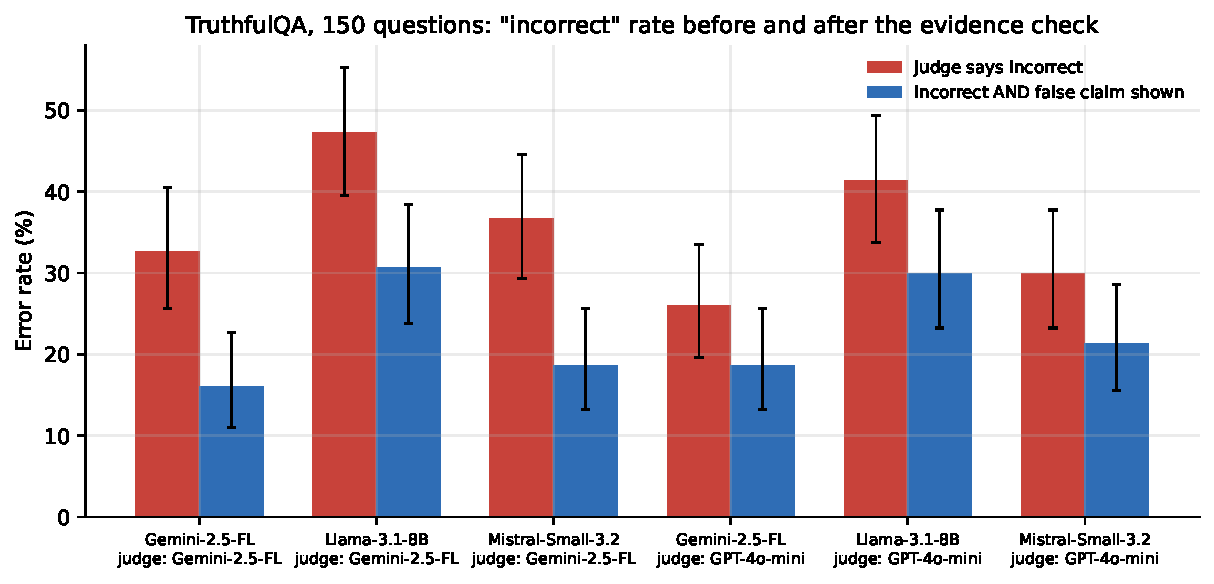
\includegraphics[width=\linewidth]{figures/fig3_evidence.pdf}
\caption{\textbf{Study B.} Raw and evidence-backed \texttt{incorrect} rates per judge and system, with 95\% Wilson intervals.}
\label{fig:current}
\end{figure}

\end{document}
